\chapter{Uncertainties and Estimation}
\label{ch:UncertandEst}

We now have a robust method for the prediction of SM background for our search for the top squark. Along with a prediction for each of the backgrounds, we need to include the systematics uncertainties for our methods. Once we incorporate them we can confirm that our methods are correct by looking at the validation regions. Finally, we can then compare the final comparisons of data-to-simulation in our SR, which will allow us to set limits on the top squark mass. 

\section{Systematic Uncertainties}\label{sec:Uncert}
We will look at the various categories of systematic uncertainties that can affect the analysis. 
\begin{itemize}
	\item \textbf{Statistical uncertainty of control regions in data}: The dominant uncertainty in data-drivel background prediction methods is generally the result of limited statistics of the control regions that are used to derive the background estimate for the signal regions.
	\item \textbf{Statistical uncertainty of simulated samples}: In some cases, the uncertainties on transfer factors derived from simulation also have a significant statistical component due to limited statistics in the simulated samples.
	\item \textbf{Uncertainties related to extrapolation from control to signal regions}: Each data-driven background estimation method relies on an extrapolation from a control region to the signal region. This leads to uncertainties specific to each method, related to the nature of the extrapolation. For instance, the LL prediction strategy uses the region with a selected lepton to estimate the background yield in the vetoes region. Appropriate correction factors are applied to both selected and vetoes regions to account for differences in the lepton selection efficiency between data and simulation. The precision of these corrections affects the uncertainty in the background estimation. For the QCD prediction, we rely on an extrapolation from the low $\Delta\phi_{12}$ region, which is mostly in the core of the jet response distribution, to a region of high values of $\Delta\phi_{12}$, which is mostly in the tail of the distribution. We therefore assign an uncertainty in the QCD precition for the potential effects of severe jet mismeasurements in the jet response tails. 
	\item \textbf{Uncertainties related to $b$-tagging}: Effects related to the $b$-tagging are estimated to impact the scale factors up to 3\% for top-jets and between 5 to 10\% for \W+jets. Uncertainties due to the top-\pt{} reweighting, pile-up, or matching criteria results to effect smaller than 3\% for both top and \W{} tags. 
	\item \textbf{Uncertainties related to the merged top and W-tagging}: The impact of different effects on the determination of the scale factors are studied. One of the dominant sources is related to the description of the parton showering which results to uncertainties of 5-25\% and 8-15\%, for top and \W{} tagging, respectively. Another source of systematics is due to the modeling of the \ttbar{} topology. The evaluated uncertainties range between 1-3\% (1-12\%) in top (\W) tagging. 
	\item \textbf{Uncertainties related to the Resolved Top Tagging}: A similar list of the sources of systematic uncertainties is evaluated for the resolved tagger, as in the case of Merged tops. The most important sources stems from the description of the parton showering, which ranges between 8-31\%. The modeling of the \ttbar{} topology can be as high as 4\%, whereas potential dependence on the $b$-tagging results to uncertainties from 1 to 6\%. Uncertainties due to the top-\pt{} reweighting, pile-up, or matching criteria results to effect smaller than 3\%. 
	\item \textbf{Luminosity}: A 2.6\% uncertainty is assigned on the integrated luminosity measured by CMS for the 2016 data-taking period. The prediction of the diboson backgrounds, which rely o simulaiton and are normalized based on the measured integrated luminosity, are affected by this uncertainty. Since the estimations of the remaining SM background processes are data-driven and based on the data observed in control regions, they are not affected by this uncertainty. 
\end{itemize}

\section{Validation}\label{sec:Validation}

\begin{table}[!ht]
\begin{center}
\caption[High $\Delta$m Search Regions]{\label{tab:validationregions-hm}Summary of the 151 disjoint search regions that mainly target high \dm~signal models. The high \dm~baseline selection is again $\nj \geq 5$, $\met>250~\GeV$, $\nb\geq1$, and $\dphijonetwothreefour>0.5$.}
\resizebox*{1\textwidth}{!}{

\begin{tabular}{|c|c|c|c|c|c|}
	\hline
	\multicolumn{6}{|c|}{$\mtb<175$\,\GeV}  \\
	\hline
	\nj				 & \nb				& \nt			   & \nw				 & \nrt				& \met~[\GeV] 		\\
	\hline
	$\geq7$		& $1, \geq2$  & $\geq0$		 & $\geq0$			& $\geq1$	  & $250-400,\geq400$ \\
	\hline
	\multicolumn{6}{|c|}{$\mtb\geq175$\,\GeV}  \\
	\hline
	\nj				 & \nb				& \nt			   & \nw				 & \nrt				& \met~[\GeV] 		\\
	\hline
	$\geq5$		& $1,\geq2$   &	$0$				& $0$				   & $0$			 & $250-400,\geq400$ \\
	\hline
	\multirow{4}{*}{$\geq5$} & \multirow{4}{*}{$1$} & $1$ & $0$ & $0$ & $250-400,\geq400$\\
						  &					   & $0$			 & $1$			& $0$			  & $250-400,\geq400$ \\
						  &					   & $0$			 & $0$				    & $1$	  & $250-400,\geq400$ \\
						  &					   & \multicolumn{3}{|c|}{$\nt+\nw+\nrt\geq3$} & $\geq400$ \\
	\hline
	\multirow{4}{*}{$\geq5$} & \multirow{4}{*}{$2$} & $1$ & $0$ & $0$ & $250-400,\geq400$\\
						  &					   & $0$			 & $1$					& $0$			& $250-400,\geq400$ \\
						  &					   & $0$			 & $0$				    & $1$	  		& $250-400,\geq400$\\
						  &					   & \multicolumn{3}{|c|}{$\nt+\nw+\nrt\geq3$} & $\geq400$ \\
	\hline
\end{tabular}
}
\end{center}
\end{table}

\begin{table}[!ht]
\begin{center}
\caption[Low $\Delta$m Search Regions]{\label{tab:validationregions-lm}Summary of the 53 disjoint search regions that mainly target low \dm~signal models. The low \dm~baseline selection is again $\nj \geq 2$, $\met>250~\GeV$, $\nt=\nw=\nrt=0$, $\nb\geq0$, $\mtb<175~\GeV$ (when applicable), $\pt(ISR) > 200$~\GeV, $ |\eta(ISR)| < 2.4$, $|\Delta\phi(j_{\text{ISR}},\met)|>2$, and $\metsig > 10$.}
\resizebox*{1\textwidth}{!}{
\begin{tabular}{|c|c|c|c|c|c|}
	\hline
	$\nj$              & $\nb$                    & $\nsv$             & $\ptisr$~[\GeV]         & $\ptb$~[\GeV]      & $\met$~[\GeV]                           \\
	\hline
	\multicolumn{6}{|c|}{\qcdlowdm}  \\
	\hline
	$2-5$              & \multirow{4}{*}{0}       & 0                  & \multirow{4}{*}{$\geq500$} & \multirow{4}{*}{-} & $250-400$ \\
	$\geq6$            &                          & 0                  &                         &                    & $250-400$ \\
	$2-5$              &                          & $\geq1$            &                         &                    & $250-400$ \\
	$\geq6$            &                          & $\geq1$            &                         &                    & $250-400$ \\
	\hline
	\multirow{5}{*}{$\geq2$} & \multirow{5}{*}{1}   & 0                  & $300-500$               & $20-40$            & $250-300$ \\
	&                          & 0                  & $300-500$               & $40-70$            & $250-300$ \\
	&                          & 0                  & $\geq500$                  & $20-40$            & $250-400$ \\
	&                          & 0                  & $\geq500$                  & $40-70$            & $250-400$ \\
	&                          & $\geq1$            & $\geq300$                  & $20-40$            & $250-300$            \\
	\hline
	$\geq2$            & \multirow{6}{*}{$\geq2$} & \multirow{6}{*}{$\geq0$} & $300-500$               & $40-80$            & $250-300$            \\
	$\geq2$            &                          &                          & $300-500$               & $80-140$           & $250-300$           \\
	$\geq7$            &                          &                          & $300-500$               & $\geq140$             & $250-300$            \\
	$\geq2$            &                          &                          & $\geq500$                  & $40-80$            & $250-400$            \\
	$\geq2$            &                          &                          & $\geq500$                  & $80-140$           & $250-400$            \\
	$\geq7$            &                          &                          & $\geq300$                  & $\geq140$             & $250-400$         \\
	\hline
	\multicolumn{6}{|c|}{\meddphi}  \\
	\hline
	$\geq2$			   & 0						& 0						   & $\geq200$					& $\geq20$			& $\geq250$		\\
	$\geq2$			   & 0						& 1						   & $\geq200$					& $\geq20$			& $\geq250$		\\
	$\geq2$			   & 1						& 0						   & $\geq200$					& $\geq20$			& $\geq250$		\\
	$\geq2$			   & 1						& 1						   & $\geq200$					& $\geq20$			& $\geq250$		\\
	\hline
	
\end{tabular}
}
\end{center}
\end{table}



In order to test and validate the background estimation strategy in data, we carry out the background estimation method in a lower \met{} region of the zero-lepton sample that is adjacent to the search sample, "low \met{} validation sample", and check the agreement between data and background prediction. The validaiton sample has significantly larger statistics than the search sample and is signal-depleted. Apart from the difference in the \met{} selection, the search selection on the other search variables is applied to the validation sample, with an exception of the regions with more than one top- or W-tags, where relaxed selections (i.e. drop selection in $M_T(b_{1,2},\met)$) are applied to gain more statistics, see Tables \ref{tab:validationregions-hm} and \ref{tab:validationregions-lm}. Figures \ref{fig:validation-region-lm} and \ref{fig:validation-region-hm} displays the SM estimate and the observed data in the different validation regions. Statistical uncertainties as well as systematic uncertainties resulting from the top- and W-tagging correction in the background predictions are shown in this plot. The data agrees well with the estimated backgrounds yields within uncertainties. 

\begin{figure}[!htb]
	\begin{center}
  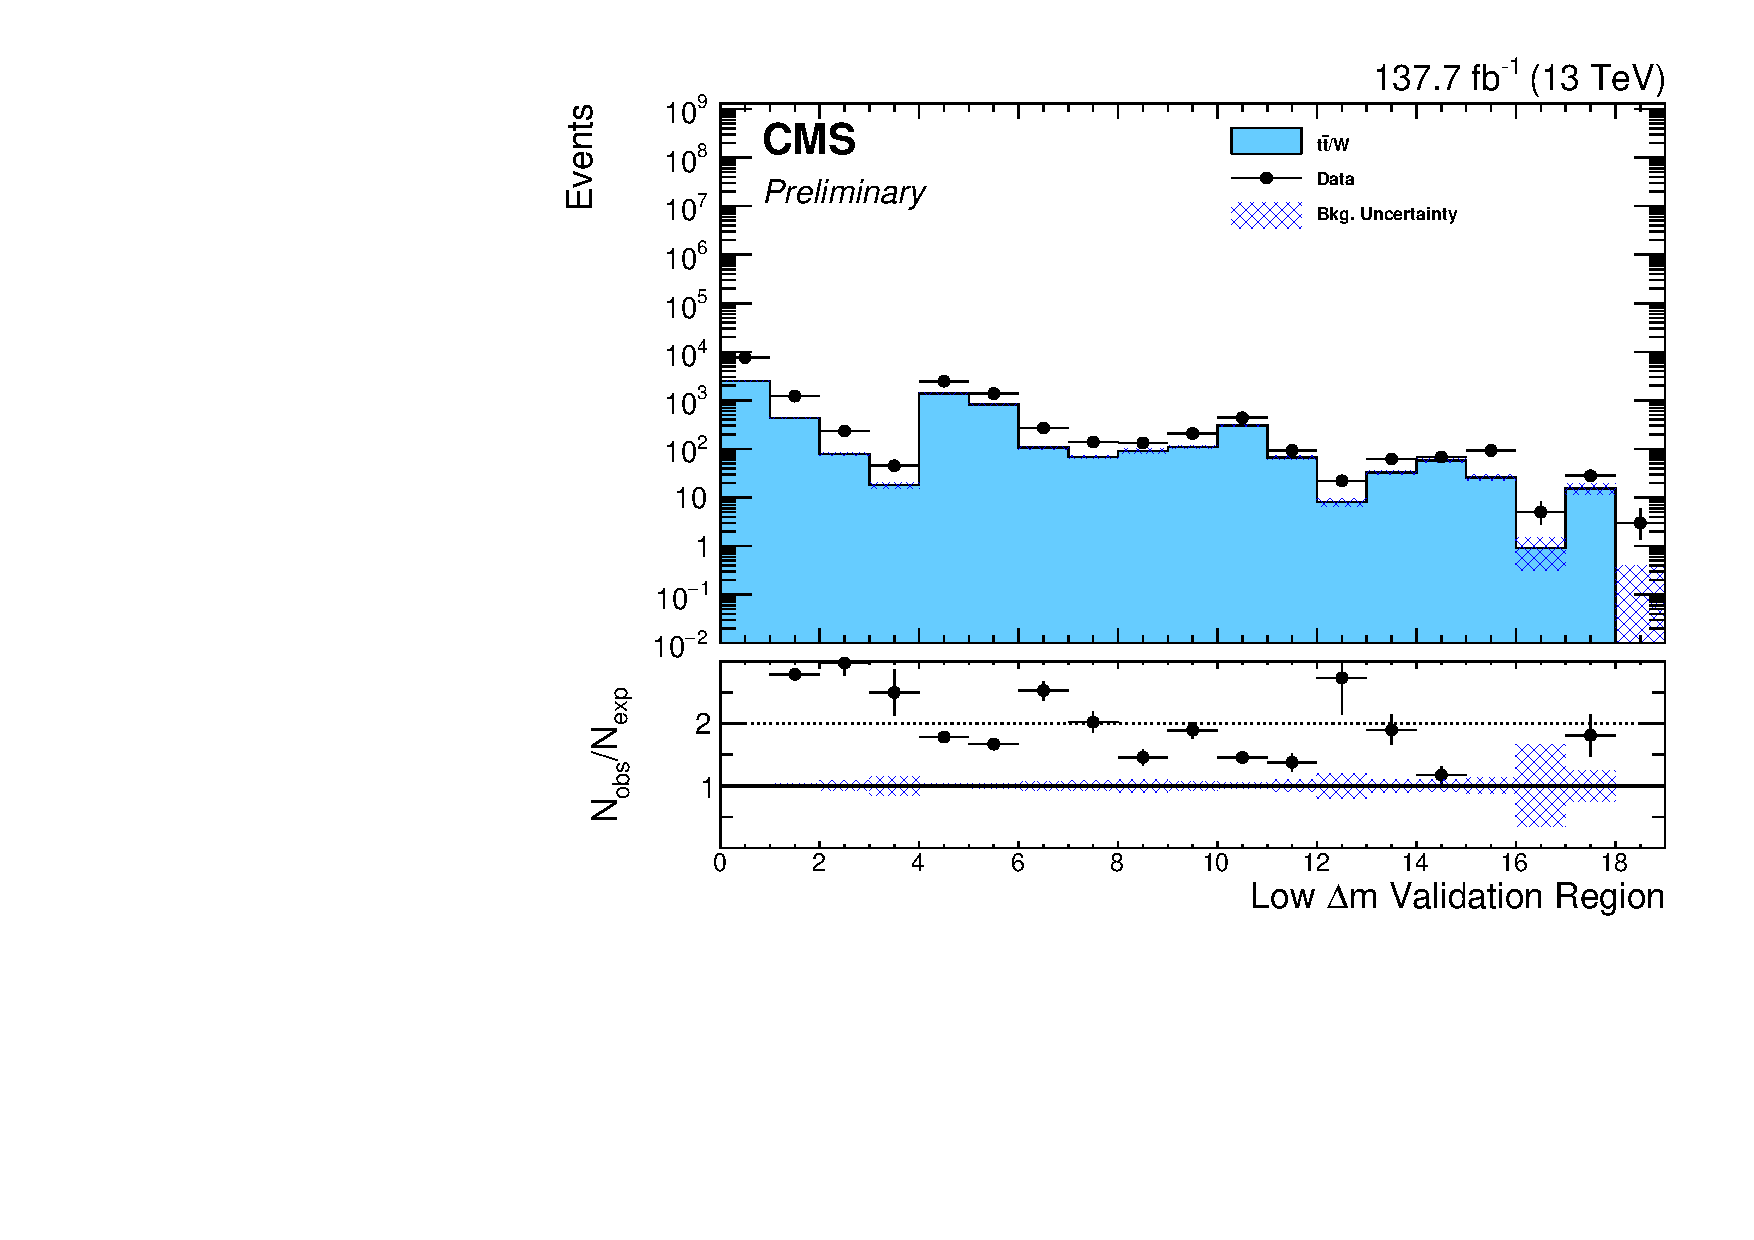
\includegraphics[width=1\textwidth]{validation_pred_LM.pdf}
	\end{center}
	\caption[LM Validation Region]{Comparison of the data and SM backgrounds in the Low \dm{} validation regions.
	 }
	\label{fig:validation-region-lm}
\end{figure}

\begin{figure}[!htb]
	\begin{center}
  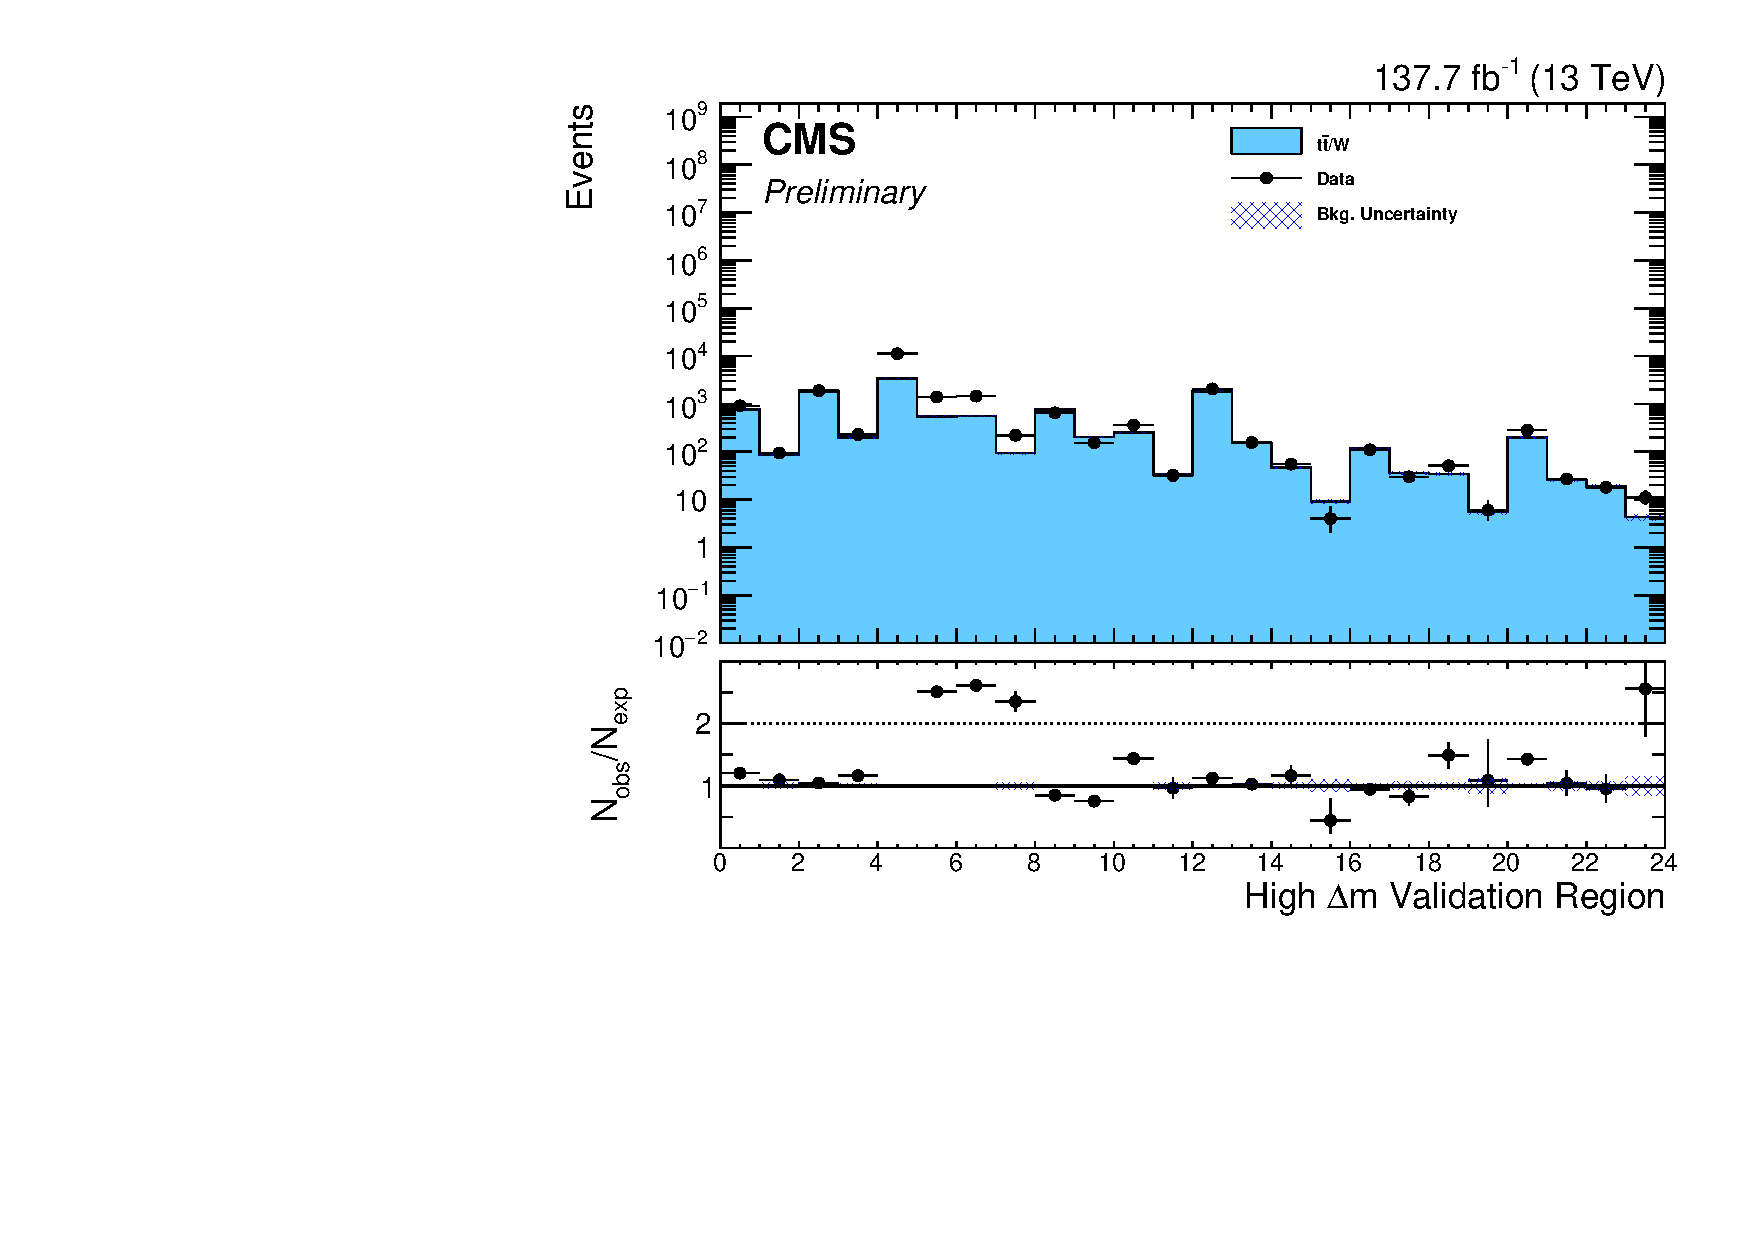
\includegraphics[width=1\textwidth]{validation_pred_HM.pdf}
	\end{center}
	\caption[Lost Lepton HM Control Region]{Comparison of the \met~distribution in the High \dm{} validation regions.
	 }
	\label{fig:validation-region-hm}
\end{figure}

Now that we have shown that the bins for the low and high \dm{} match well with data we can move to a full comparison of the data and simulation in the SR. To do this we combine the predictions from the LL, \Znunu, QCD, and Rare backgrounds. We need to 